The relationship between the 16$^{th}$, 50$^{th}$ and 84$^{th}$ fractiles of $\mu$ and R needs to be drawn, as represented in Figure~\ref{fig:Rmu}. This is done by computing $\beta_{\theta d}$ for a discretised number of R with eq. \ref{eq:beta_eq_RGM}, and obtaining from this value the 16$^{th}$ and 84$^{th}$ fractiles of $\mu$ ($\mu_{16\%}$ and $\mu_{84\%}$), according to the Equations~\ref{eq:mu16-beta} and \ref{eq:mu84-beta}.

\begin{figure}[!htbp]
\centering
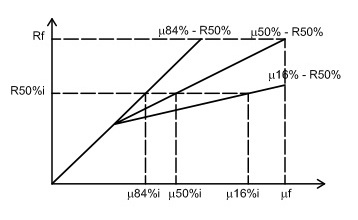
\includegraphics[width=8cm]{figures/Rmu.jpg}
\caption{R-$\mu$ relationship.}
\label{fig:Rmu}
\end{figure}

\begin{equation}
\mu_{ds,16} = \hat{\mu}_{ds} e^{-\beta_{\theta d,ds}}
\label{eq:mu16-beta}
\end{equation}
\begin{equation}
\mu_{ds,84} = \hat{\mu}_{ds} e^{\beta_{\theta d,ds}}
\label{eq:mu84-beta}
\end{equation}

The median $R_{50\%}$ values have been already computed with Equation~\ref{eq:R_RGM}, and $\mu_{16\%}$-$R_{50\%}$, $\mu_{50\%}$-$R_{50\%}$ and $\mu_{84\%}$-$R_{50\%}$ curves can now be drawn.

If uncertainty in the damage criteria $\beta_{\theta c}$ is equal to 0 the $R_{50\%}$, $R_{16\%}$, and $R_{84\%}$ values corresponding to the ductility limit states $\mu_{ds}$ are found interpolating the aforementioned R-$\mu$ curves, and converted into $\hat{S}_{a,ds}$ and $\beta_{S_{a d}}$ according to the following equations:

\begin{equation}
\hat{S}_{a,ds} = R_{50\%}(\mu_{ds}) S_{ay}
\label{eq:SaR}
\end{equation}
\begin{equation}
\beta_{S_{a d}} = \beta_{R(\mu)} = \frac{\ln R(\mu)_{84\%} - \ln R(\mu)_{16\%}}{2}
\label{eq:betaR}
\end{equation}

where
\begin{equation}
S_{ay} = \frac{4 \pi^2 d_{roof,y}}{T_1^2 g \Gamma_1}
\label{eq:Say}
\end{equation}

If $\beta_{\theta c}$ is different from 0 instead, different values of ductility limit state are sampled from the lognormal distribution with median the median value of the ductility limit state, and dispersion the input $\beta_{\theta c}$.
For each of these ductilities the corresponding $R_{50\%}$, $R_{16\%}$, and $R_{84\%}$ values are found interpolating the aforementioned curves, and converted into $\hat{S}_{a,ds}$ and $\beta_{S_{a d}}$ according to Equations \ref{eq:SaR} and \ref{eq:betaR}.

MC random S$_a$ for each of the MC sampled ductility limit states are computed using $\hat{S}_{a,ds}$ and $\beta_{S_{a d}}$, and their median and dispersion are estimated. These parameters constitute the median $\hat{S}_{a,ds}$ and the total dispersion $\beta_{S_a}$ for the considered damage state. The procedure is repeated for each damage state.

\subsubsection{Multiple-Building Fragility and Vulnerability function}
\label{subsubsec:multiple-buildings}
If multiple buildings have been input to derive fragility function for a class of buildings all $\hat{S}_{a, blg}$ and $\beta_{S_a, blg}$ are combined in a single lognormal curve. A minimum of 5 buildings should be considered to obtain reliable results for the class.\\ 
A new issue arises when multiple buildings are considered: the S$_a$ at the fundamental period of each building should be converted to a common intensity measure, to be able to combine the different fragility functions. A common intensity measure is selected to be S$_a$ at the period T$_{av}$, which is a weighted average of the individual building fundamental periods T$_1$. Then each individual fragility needs to be expressed in terms of the common S$_a$(T$_{av}$), using a spectrum. FEMA P-695 far field set of 44 accelerograms (22 records for the two directions) was used to derive a mean uniform hazard spectrum, and the ratio between the S$_a$ at different periods is used to scale the fragility functions. It can be noted that the actual values of the spectrum are not important, but just the spectral shape.

The median $\hat{S}_a$ is converted to the mean $\mu_{ln(S_a)}$ of the corresponding normal distribution ($\mu_{ln(S_a)} = ln(\hat{S}_a)$) and, simply scaled to the common intensity measure as follows:

\begin{equation}
\mu_{ln(S_a), blg} = \mu_{ln(S_a), blg} S(T_{av})/ S(T_{1, blg})
\end{equation}
\begin{equation}
\beta_{S_a, blg} = \beta_{S_a, blg} S(T_{av})/ S(T_{1, blg})
\label{eq:Sa(Tav)}
\end{equation}

Finally the parameters of the single lognormal curve for the class of buildings, mean and dispersion, can be computed as the weighted mean of the single means and the weighted SRSS of the inter-building and intra-building standard deviation, the standard deviation of the single means and the single dispersions respectively, as shown in the following equations:

\begin{equation}
\mu_{ln(S_a), tot} = \sum_{i=0}^{n.blg} w_{blg-i} \mu_{ln(S_a), blg-i}
\label{eq:combination-lognormals-mu}
\end{equation}
\begin{equation}
\beta_{S_a, tot} = \sqrt{ \sum_{i=0}^{n.blg} w_{blg-i} ((\mu_{ln(S_a), blg-i}-\mu_{ln(S_a), tot})^2+ \beta_{S_a, blg-i}^2})
\label{eq:combination-lognormals-sigma}
\end{equation}

The mean $\mu_{ln(S_a)}$ and total dispersion $\beta_{S_a}$ of the fragility function of the class are converted to logarithmic mean $\mu_{S_a}$ and logarithmic covariance $cov_{S_a}$ (standard deviation $\sigma_{S_a}$ over $\mu_{S_a}$), according to the following equations:

\begin{equation}
\hat{S}_a = e^{\mu_{ln(S_a)}}
\end{equation}
\begin{equation}
\mu_{S_a} = \hat{S}_a e^{\frac{\beta_{S_a}^2}{2}}
\label{eq:median-to-mean}
\end{equation}
\begin{equation}
\sigma_{S_a} = \sqrt[2]{(\beta_{S_a}^2-1) e^{2\ln{ \hat{S}_a}+\beta_{S_a}^2}}
\label{eq:dispersion-to-standard}
\end{equation}
\begin{equation}
cov_{S_a} = \frac{\sigma_{S_a}}{\mu_{S_a} }
\end{equation}